
\bbsubsection{Currency Selection}{add-account-currency}

The currency selection screen enables users to search and select a currency to use for their new account. The user can search for the country's name, the currency name, or the currency symbol through the search bar. Once the user is satisfied with their selection, they can tap the Back button to return to the Add New Account screen, where they will see their newly selected currency in the Currency Cell (Item \#4 of the \nameref{add-account-currency-screenshots} section).

\bbsubsubsection{Application Screenshots}{add-account-currency-screenshots}

\begin{figure}[h]
 
\begin{subfigure}{0.5\textwidth}
  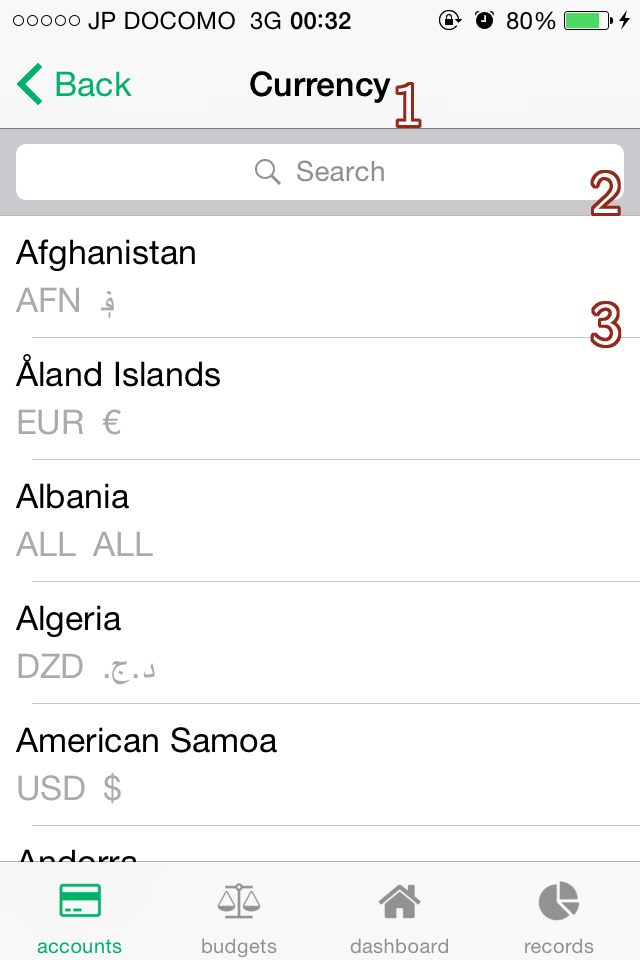
\includegraphics[scale=0.35]{ACC-0001-3} 
  \caption{Currency Selection Screen}
  \label{fig:currency-1}
\end{subfigure}
\begin{subfigure}{0.5\textwidth}
  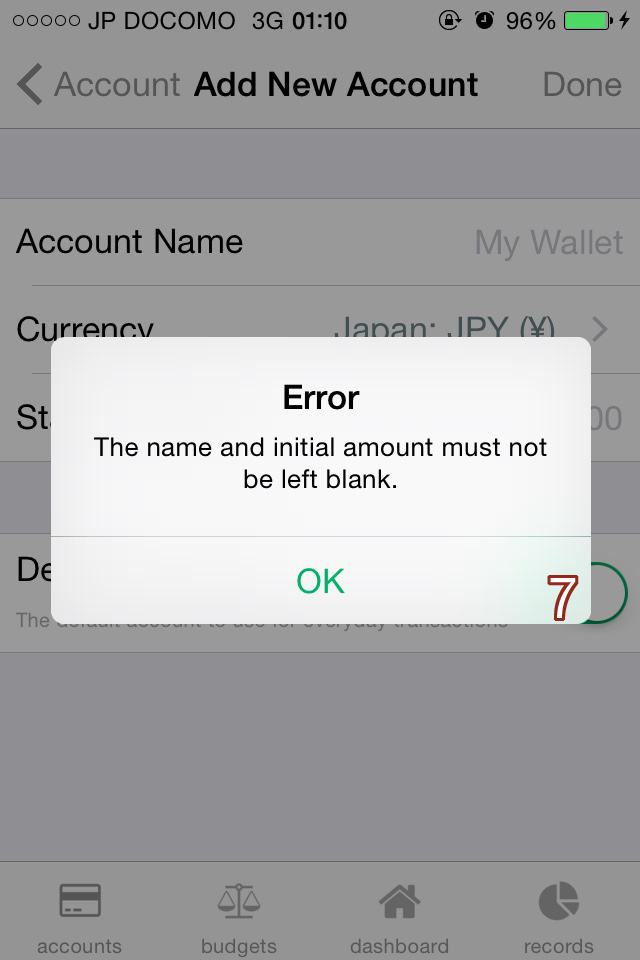
\includegraphics[scale=0.35]{ACC-0001-4}
  \caption{Currency Loading Screen}
  \label{fig:currency-2}
\end{subfigure}
\caption{Currency Selection Screenshots}
\label{Currency Selection Screenshots}
\end{figure}

\screentable{
	\header{Screen Component}
    	{Type} 
        {Description}
    \row{1. Screen Title}
    	{Label Title}
        {Localization Key: MENULABEL\_CURRENCY\_PICKER}
    \row{2. Search Field}
    	{Search Bar}
        {When tapped, a QWERTY keyboard is displayed, and the search textfield is given focus. \doublenewline
        
        At the same time, the width of the textfield shortens, giving way to the Cancel button which, when tapped, dismisses the keyboard and returns it to the state shown in the screenshot.\doublenewline
        
        Note that because the search bar is placed at the header of the table, it will move together as the user scrolls and it is not fixed on the top of the screen. 
        } 
        
    \row{3. Loading Screen}
    	{Label}
        {This label is displayed while the currency data is being loaded. \doublenewline
        
        While loading, the user cannot scroll.\doublenewline 
        
        Localization Key: GUIDELABEL\_LOADING
        } 
        
    \row{4. Currency Selection Cell}
    	{Table Cell}
        {This table cell consists of three UI labels showing the currency's country, code, and symbol. \doublenewline
        
        Tap anywhere in the cell and a checkmark will appear on its right side, indicating that a type of currency has been selected.
        } 
}